\section{提案するサーバテスト手法}

\subsection{テスト種別の選択}

2章にて,従来のテスト手法では構成管理ツール独立性とOS・ディストリビューション汎用性の双方を満たすものが,どのテスト種別においても存在しない,ということを述べた.そこでまず,本論文で提案する手法を,どのテスト種別に適用するのか選択を行う.

種別(1)の単体テストは既に述べたように,サーバのテスト手法としては不十分である.また,構成管理ツール固有の言語により書かれたコードをテストするものなので,構成管理ツールから切り離して考えることができない.よって単体テストは提案手法の対象から除外する.種別(3)の受け入れテストは,サーバの外からの振る舞いをテストするもので,内部状態をテストするものではない.サーバ構成を記述したコードのテストは,コードによってもたらされたサーバ内部の設定状態をテストすべきものと考える.よって受け入れテストは提案手法の対象から除外する.残る種別(2)の結合テストは,サーバの内部状態を網羅的にテスト可能であり,サーバ構成を記述したコードのテストとして相応しいものである.よって(2)の結合テストを提案手法の適用対象とする.

\subsection{要件の考察}

次に,結合テストにおいて構成管理ツール独立性とOS・ディストリビューション汎用性の双方を満たすための要件について考察する.

特定の構成管理ツールからの独立性を満たせない理由は二つある.一つは,テストスイートはテストに必要なプロセスをすべて実行するため,テスト用VMを構築する機能も併せ持つが,この機能が特定の構成管理ツールを用いてVMを構築することが前提となっているためである.もう一つは,テストコードにOS・ディストリビューション汎用性を持たせるために,構成管理ツールが元々持っているOSの違いを吸収する機能に実装が依存しているためである.

OS・ディストリビューション汎用性が満たせないのは,テストがシェルコマンドを直接記述する実装になっており,OS・ディストリビューションの違いをテストコードを書く者自らが意識しないといけないからである.この考察から,提案するテスト手法に必要な要件は以下の通りとなる.

\begin{enumerate}
  \item テストスイートではなくテストのみに特化する
  \item テストの実装を特定の構成管理ツールに依存しない
  \item OS・ディストリビューションの違いをテストコードを書く者に意識させない
\end{enumerate}

\subsection{要件を満たすための手法の提案}

考察した要件を満たすために,運用業務で発生するコマンド群,特に確認作業に必要なコマンド群の体系化・抽象化を行う.そのためにまずはOS・ディストリビューション毎にコマンドを分離し,統一的なAPIでコマンドを呼び出すことができる汎用コマンド実行フレームワークを定義する.次に,汎用コマンド実行フレームワークを宣言的かつ自然言語に近い記法で操作できる制御テストフレームワークを定義する.汎用コマンド実行フレームワークと制御テストフレームワークの仕組みおよびその関係を\figref{fig:framework}に示す.汎用コマンド実行フレームワークではまず,構成管理ツール固有の振る舞い(パッケージインストール等)を抽出する.そして要件(1)を満たすために,振る舞いのテストに特化したAPIを定義する.更にAPIから呼び出されるコマンドをOS・ディストリビューション毎に定義し,要件(2)を満たすために,APIとコマンド群の間にはOS・ディストリビューションを判別して自動で適切なコマンドを返すレイヤーを設ける.ここは構成管理ツール等,特別なソフトウェアを必要としない方式をとる.制御テストフレームワークではまず,要件(3)を満たすため,テストコード記述の抽象度を高め可読性を上げるために,宣言的かつ自然言語に近い記法で汎用コマンド実行フレームワークを操作するための記法の定義を行う.次に記法内の各命令と実際に呼び出す汎用コマンド実行フレームワークのAPIメソッドをひもづける.



\begin{figure}[tb]
  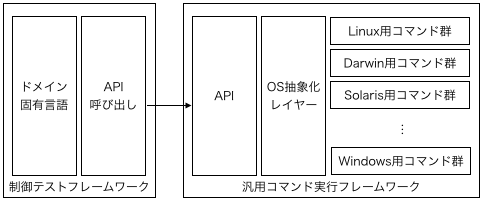
\includegraphics{framework-overview.png}
  \caption{汎用コマンド実行フレームワークと制御テストフレームワークの仕組みと関係}
  \label{fig:framework}
\end{figure}

\subsection{提案手法の実装}

提案手法に基づき実装した汎用コマンド実行フレームワークをspecinfra\cite{specinfra},制御テストフレームワークをserverspec\cite{serverspec}と名付けた.specinfra,serverspecともに実装にはRubyを採用している.Rubyを採用した理由はRSpecを利用するためである.RSpecはテストフレームワークとして実績があり,自然言語に近い形でテストコードを記述することができるという要件を満たし,記法の拡張が可能であることから採用した.

\begin{figure}[tb]
\setbox0\vbox{
\begin{verbatim}
describe file("/etc/password") do
  it { should be_file }
end

describe file("/tmp") do
  it { should be_directory }
end

describe file("/var/run/unicorn.sock") do
  it { should be_socket }
end

describe file("/etc/httpd/conf/httpd.conf") do
  its(:content) do
    should match /ServerName www.example.jp/
  end
end
\end{verbatim}
}
\centerline{\fbox{\box0}}
\caption{serverspecによりファイルをテストするためのコード\label{fig:test-files-with-serverspec}}
\end{figure}

\begin{figure}[tb]
\setbox0\vbox{
\begin{verbatim}
describe user("root") do
  it { should exist }
  it { should have_uid 0 }
  it { should belong_to_group "root" }
  it { should have_home_directory "/root" }
  it { should have_login_shell "/bin/bash" }
end

describe group("root") do
  it { should exist }
  it { should have_gid 0 }
end
\end{verbatim}
}
\centerline{\fbox{\box0}}
\caption{serverspecによりシステムユーザ/グループをテストするためのコード\label{fig:test-users-with-serverspec}}
\end{figure}

RSpecを採用することによりテストコードがどのように書けるのかを例で示す.\figref{fig:test-files-with-serverspec}にserverspecによりファイルに対してテストを行うためのコードを示す.describeではテストの対象となるサーバ上のリソースを指定する.この図ではfile("/etc/passwd")などがそれにあたる.これによりテスト対象が/etc/passwdというファイルであることを指定する.テストしたい内容はit \{ should ... \}といった形で記述する.例えば,it \{ should be\_file \}は,対象リソースがファイルとして存在する,ということをテストするためのコードである.また,its(:content)といった形で指定することで,対象リソースそのものだけではなく,リソースに付随するもの,この例ではファイルの内容についてもテストすることができる.

\figref{fig:test-users-with-serverspec}にシステムユーザ/グループに対してテストを行うためのコードを示す.この例では,rootユーザが存在し,uidが0,rootグループに所属,ホームディレクトリが/root,ログインシェルが/bin/bashであること,rootグループが存在し,gidが0であることをテストしている.

\subsection{serverspecの特徴}

提案手法に基づき実装したserverspecの特徴について述べる.特徴の一つとして,特定の構成管理ツールに依存していないことが挙げられる.そのため,どの構成管理ツールを利用していてもserverspecを利用することができる.それだけにとどまらず,構成管理ツールを利用していない場合でもserverspecを利用することができる.ゆえに特定の構成管理ツール依存のテストツールと比べて利用の間口が広いと言える.また,特定の構成管理ツールに依存していないということは,テスト対象のサーバに特定のソフトウェアを入れる必要がないということでもある.serverspecはテスト対象サーバでsshdが動いてさえいれば,Rubyすら入れる必要がない.そのため特定の構成管理ツール依存のテストツールと比較して利用の敷居が低い.

二つ目の特徴はTest Kitchenやrspec-systemのような統合テストスイートと比較して単機能な点である.単機能であるため他のツールとも組み合わせやすく,同種ツールとしてとりあげたTest Kitchenやrspec-systemには,ツール標準のテスト機構をserverspecで置き換えるためのプラグインや,Vagrant\cite{vagrant}と連携してVMのテストを行うプラグインが存在する.

三つ目の特徴は記法の汎用性と抽象度の高さである.汎用性を高めたため,OS・ディストリビューションの違いを気にすることなくテストを容易に書くことができる.また抽象度が高いためテストコードの可読性が高く,メンテナンス性が高い.
